\section{Running a Kernel}
To run a kernel, the host program runs the \verb/run_kernel/ function with a reference to the kernel pointer, as well as the number of threads it wants to spawn.
Listing \ref{lst:run-kernel} shows the code required for running a kernel.

\begin{c-code}[caption=Running a kernel, label=lst:run-kernel]
run_kernel(fill_screen, 4096);
\end{c-code}

\begin{figure}[H]
    \centering
    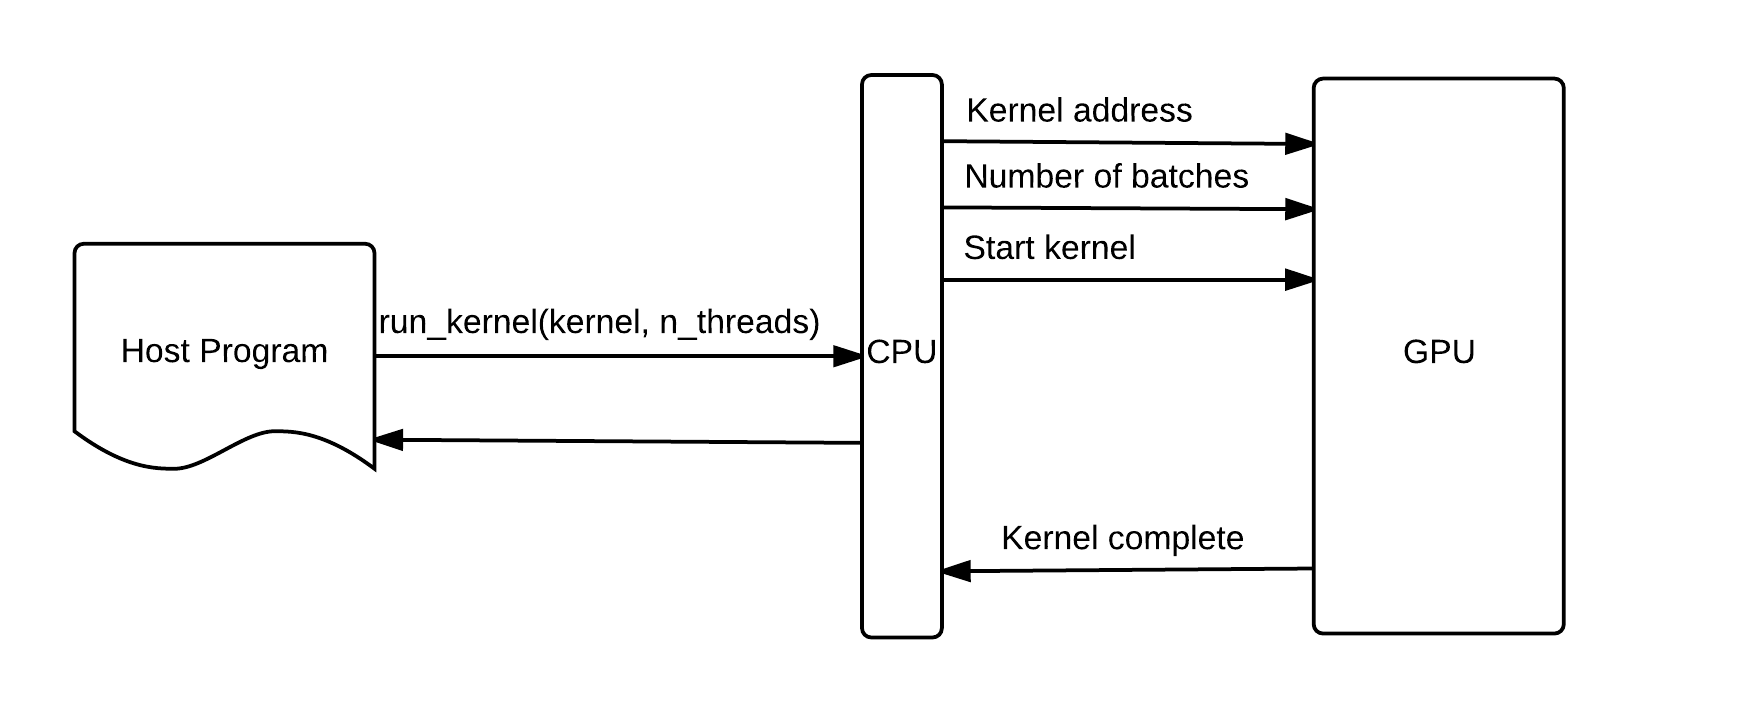
\includegraphics[width=\textwidth]{../cpu/diagrams/running_a_kernel.png}
    \caption{Starting a kernel on the GPU.}
    \label{fig:running_a_kernel}
\end{figure}

Telling the GPU to start executing a kernel is accomplished by writing the number of threads to spawn to the address of the first instruction.
Because of the 16-bit size of the data bus, the maximum number of threads would be limited to 65536.
What is actually written is the number of batches of threads to spawn.
A batch is the number of threads which is simultaneously executing across all processor cores on the GPU.
To separate this from an actual instruction upload, an address offset is used,
effectively asserting the 18th bit of the address line (figure \ref{fig:start_kernel_format}).

\begin{figure}[H]
    \centering
    \begin{tabular}{|c|c|c|c|}
    \multicolumn{1}{c}{1} & \multicolumn{1}{c}{1} & \multicolumn{1}{c}{2} & \multicolumn{1}{c}{16} \\ \hline
    X & 1 & 00 & address \\ \hline
    \end{tabular}
    \caption{Address format for starting a kernel.}
    \label{fig:start_kernel_format}
\end{figure}

The \verb/run_kernel/ call will block until the kernel has completed execution.
